\chapter{Domainanalyse}

\section{Konzeptionelles Modell}

\begin{figure}[H]
  \begin{center}
    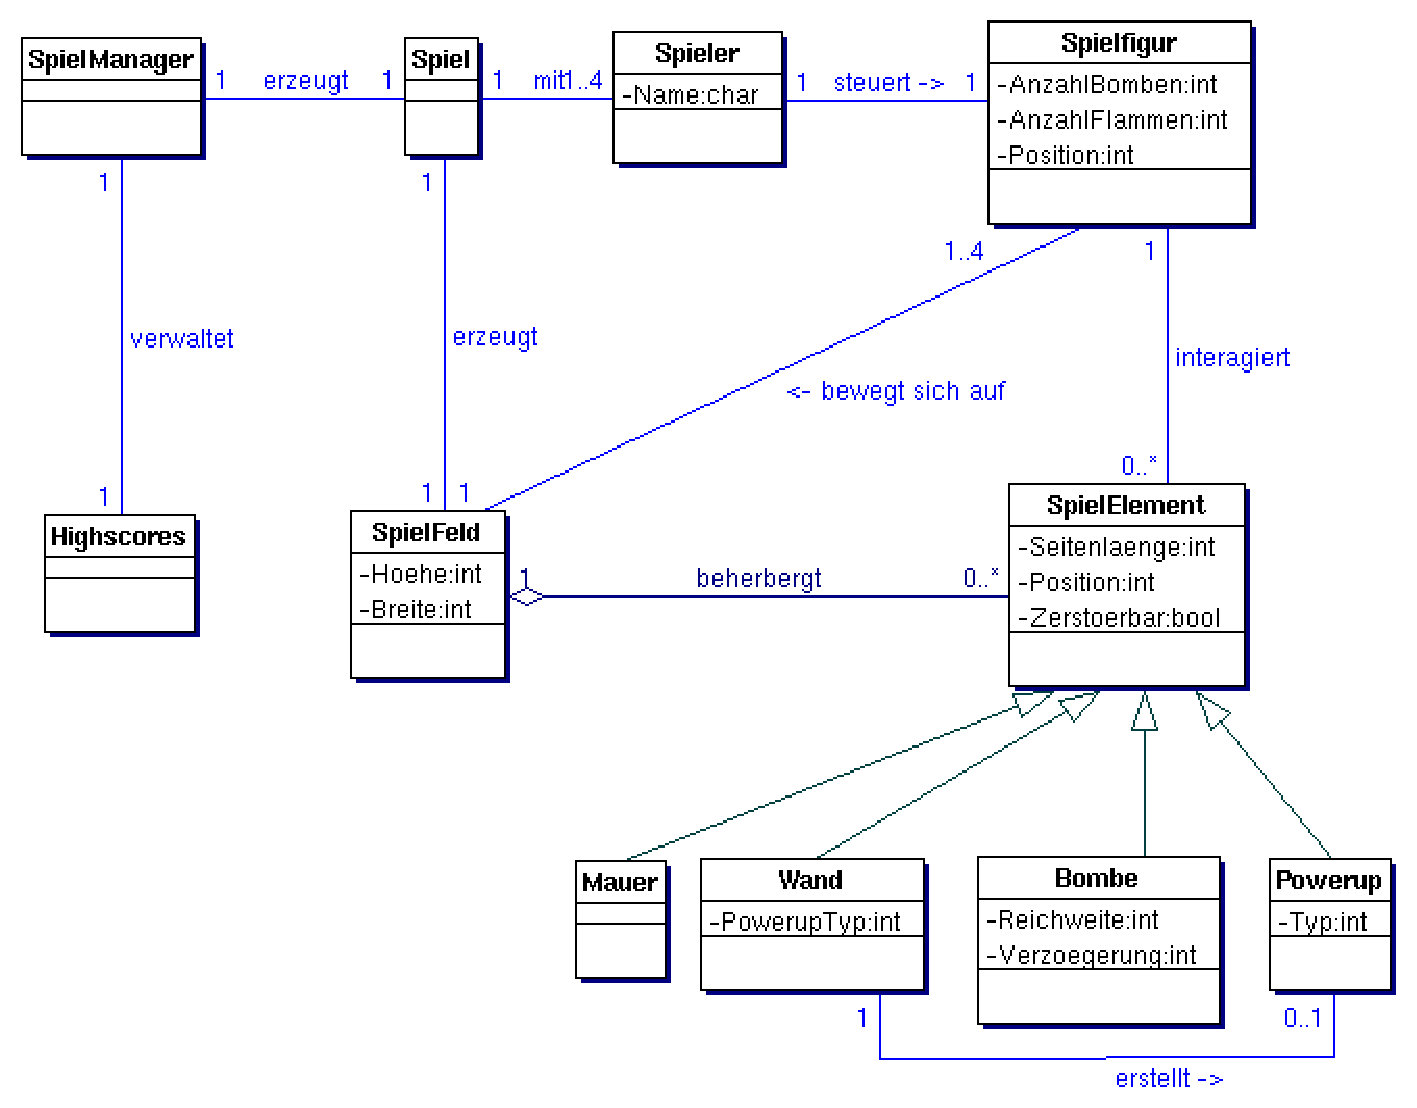
\includegraphics[width=14cm]{./images/domainmodell.pdf}
  \end{center}
  \caption{Domainmodell}
\end{figure}

\subsection{Spielmanager}
Der SpielManager ist f"ur die Initialisierung des Spiels zust�ndig. Er kennt die zwei Spieler und weitere f"ur das Spiel
notwendige Parameter.

\subsection{Spiel}
Das Spiel erzeugt das Spielfeld und positioniert die Spielelemente f"ur den Start des Spiels.

\subsection{Spielfeld}
Das Spielfeld ist der Hintergrund auf dem das eigentliche Spiel stattfindet. Es hat eine bestimmte H"ohe und Breite die zu beginn
festgelegt werden. Auf dem Spielfeld befinden sich die Objekte des Spielfeldes:Spielelemente und Spielfigur. Alle Objekte
des Spielfeldes haben eine Position. Das Spielfeld kennt alle Objekte und ihre Positionen.

\subsection{Spielelement}
Das Spielelement dient als Oberklasse f"ur s"amtliche sich auf dem Spielfeld befindlichen Objekte, ausser der Spielfigur.
Die einheitliche Schnittstelle erleichtert die Realisierung einiger Funktionen wie die Zerst"orung von Objekten usw.
Ein Objekt des Spielfeldes belegt normalerweise ein Feld auf dem Spielfeld.
Es kann "uber das Spielfeld die Belegung der benachbarten Felder abfragen.

\subsection{Spielfigur}
Die Spielfigur ist das einzige Objekt des Spielfeldes das sich auf dem Spielfeld bewegen kann. Sie kann mit den Spielelementen
kommunizieren. Die Spielfigur kann zum Beispiel Bomben erzeugen (legen) oder Powerups aufnehmen. Andererseits wird sie
von Mauern und W"anden am weitergehen gehindert.

\subsection{Mauer}
Die Mauer wird vor Spielbeginn erzeugt und bleibt w"ahrend dem ganzen Spiel an ihrem Platz. Sie kann nicht zerst"ort werden, trotzt
also auch explodierenden Bomben.

\subsection{Wand}
Die Wand wird ebenfalls zu beginn erzeugt, kann aber durch Bomben gesprengt werden und verschwindet in diesem Fall vom Spielfeld.
Eine Wand kann (muss aber nicht) ein Powerup beherbergen. Dieses bleibt auf dem Feld liegen falls die Wand zerst"ort wird.

\subsection{Bombe}
Die Bombe wird von der Spielfigur erzeugt. Dabei werden die Attribute wie Reichweite und Verz"ogerungszeit gesetzt. Danach ist
die Bombe ein eigenst"andiges Spielelement und explodiert entweder nach Ablauf der Verz"ogerungszeit oder wenn sie von einer
anderen Bombe gesprengt wird. Nach dem Explodieren meldet sie ihr Ableben der Spielfigur, die sie erzeugt hat.

\subsection{Powerup}
Ein Powerup ist entweder vom Typ Bombe (eine Bombe mehr in serie) oder vom Typ Flamme (gr"ossere Reichweit) und ist zu Beginn
unter einer Wand verborgen. Es tritt erst in erscheinung wenn die Wand durch eine Bombe zerst"ort wurde.
Betritt eine Spielfigur dasselbe Feld, nimmt sie das Powerup auf und es wird gel"oscht. Wird das Powerup von einer explodierenden
Bombe erfasst, wird es zerst"ort.

\subsection{Spieler}
Der Spieler hat einen Namen und steuert die Spielfigur. Er kann sie in alle 4 Richtungen bewegen und Bomben legen.
